\section{Présentation}
	L'algorithme des fuzzy c-means se fait en plusieurs étapes. On initialise tout d'abord les degrés d'appartenance de chaque point à chaque classe. Cela peut se faire de manière aléatoire ou en appliquant la binarisation par seuillage présentée précédemment. On procède ensuite par itération pour mettre à jour ces degrés d'appartenance. Une itération se déroule de la façon suivante :\\

	\begin{itemize}
		\item on calcule pour chaque classe la moyenne des intensités pondérée par les degrés d'appartenance;
		\item on calcule la distance entre chaque pixel et ces moyennes pondérées;
		\item on met à jour le degré d'appartenance de chaque pixel à chaque classe en prenant en compte toutes ces distances.
	\end{itemize}
	\bigskip

	Le degré d'appartenance est compris entre 0 et 1. Plus il est proche de 1 et plus on est sûr que le pixel appartient à la classe. Dans le calcul de la mise à jour des degrés d'appartenance, un paramètre que l'on appelle indice de flou entre en jeu. On répète les itérations jusqu'à ce que la fonction de coût ne change plus.\\

	Dans cet algorithme nous avons plusieurs choix et paramètres : tout d'abord l'initialisation, qui peut se faire de différentes manières, et l'indice de flou. Nous allons étudier l'influence des ces différents choix sur nos résultats.

\section{Résultats}

	\subsection{Avec une initialisation par binarisation} % (fold)
	\label{ssub:avec_une_initialisation_par_binarisation}
		Nous allons tout d'abord appliquer l'algorithme des fuzzy c-means avec un indice de flou de 2 (c'est celui qui est généralement utilisé) et une initialisation basée sur la binarisation par seuillage. Notre fcm sera effectué avec 3 classes, représentant :
		\begin{itemize}
			\item la tumeur;
			\item le reste du cerveau;
			\item le fond.
		\end{itemize}

		\begin{figure}[H]
			\centering
			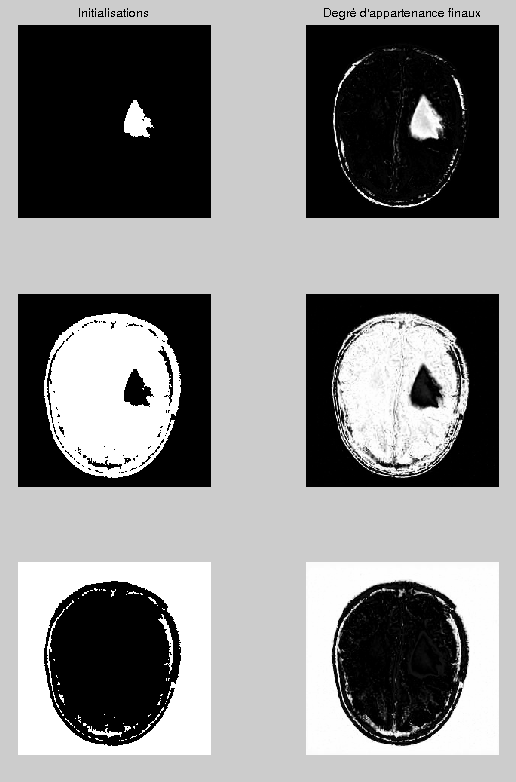
\includegraphics[height=\textheight]{images/2-fcm_bin.png}
			\caption{Degrés d'appartenance initiaux et finaux aux trois classes}
			\label{fig:fcm_avec_binarisation}
		\end{figure}

		Nous utilisons un seuil de 0.1 pour le cerveau et un seuil de 0.4 pour la tumeur.\\

		Nous appliquons ensuite l'algorithme des fcm afin de faire varier les degrés d'appartenances des pixels à chaque classe. Nous nous arrêtons lorsque les variations de la fonction de coût sont inférieures à $10^{-8}$. Cela prend une trentaine d'itérations pour chaque image, ce qui correspond à 1,53 secondes de calcul.

		La figure \ref{fig:fcm_avec_binarisation} présente dans la colonne de gauche les degrés d'appartenance initiaux pour les classes correspondant (de haut en bas) à la tumeur, au cerveau et au fond; et dans la colonne de droite les degrés d'appartenance finaux à ces mêmes classes.\\

		Il nous suffit ensuite d'attribuer à chaque pixel la classe pour laquelle son degré d'appartenance est le plus grand. On remarque qu'encore une fois, d'autres zones que la tumeur ont été labellisées comme appartenant à cette classe. Comme pour la binarisation, on dit que la tumeur correspond à la zone de cette classe ayant la plus grande surface. On obtient alors le résultat présenté en figure \ref{fig:fcm_tumeur} pour l'IRM avant traitement.

		\begin{figure}[H]
			\centering
			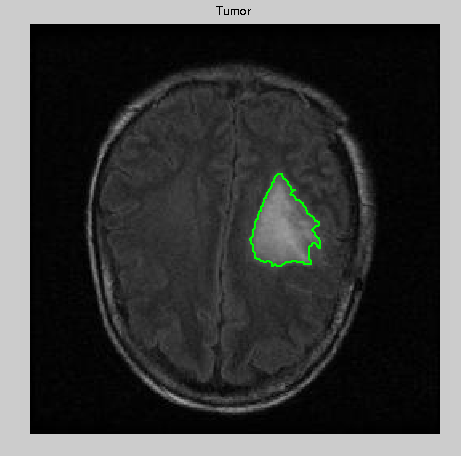
\includegraphics[width=0.5\textwidth]{images/2-tumeur.png}
			\caption{Contours de la tumeur}
			\label{fig:fcm_tumeur}
		\end{figure}

		En appliquant cette technique sur les deux IRMs, on obtient un diminution de la tumeur de 6,23\%.
	% subsection avec_une_initialisation_par_binarisation (end)

	\subsection{Avec une initialisation aléatoire} % (fold)
	\label{ssub:avec_une_initialisation_al_atoire}
		Nous allons appliquer l'algorithme des fuzzy c-means avec les mêmes paramètres que précédemment (indice de flou de 2 et les même 3 classes) mais avec une initialisation aléatoire. Cette fois-ci l'algorithme effectue entre 40 et 50 itérations en 1,39 secondes. \\

		\begin{figure}[H]
			\centering
			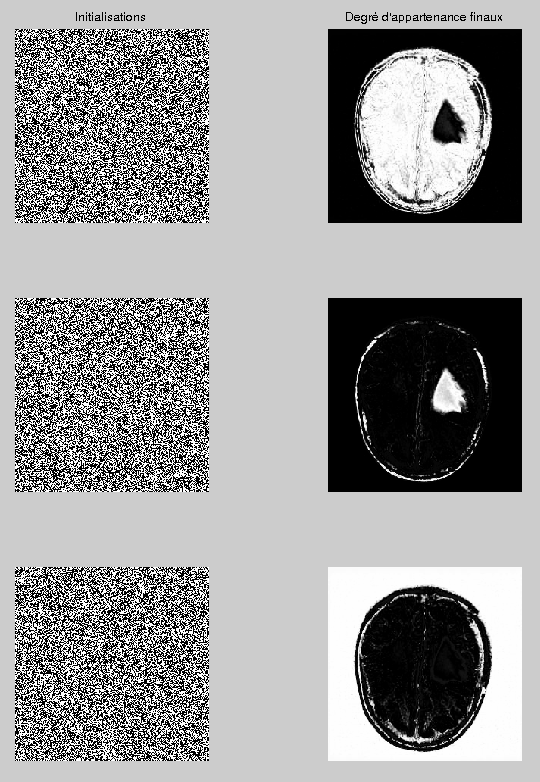
\includegraphics[height=\textheight]{images/2-rand_init.png}
			\caption{Degrés d'appartenance initiaux et finaux aux trois classes}
			\label{fig:fcm_rand}
		\end{figure}

		Il est logique d'effectuer un plus grand nombre d'itérations: l'initialisation étant aléatoire, il faut mettre à jour plus de fois les degrés d'appartenance avant que l'algorithme ne converge. L'algorithme est cependant plus rapide car l'initialisation aléatoire est bien plus rapide que l'initialisation par binarisation, qui demande d'appliquer la binarisation à deux reprises.\\

		La figure \ref{fig:fcm_rand} présente dans la colonne de gauche les degrés d'appartenance initiaux (donc aléatoires) pour les 3 classes; et dans la colonne de droite les degrés d'appartenance finaux à ces mêmes classes.\\

		Étant donné que l'initialisation est aléatoire, on ne sait pas directement quelle classe correspond à quelle partie de l'image (tumeur, cerveau ou fond). Pour cela on fait les moyennes des intensités des pixels de chaque classe, et on dit que la classe correspondant à la tumeur est celle dont la moyenne des intensités est plus élevée, puisque cette zone est la plus claire de l'image.\\

		Après avoir attribué les classes et gardé uniquement la tumeur en nous basant sur l'aire, nous obtenons les contours de la tumeur, présentés en figure \ref{fig:fcm_tumeur_rand}. La diminution de tumeur obtenue est de 6,23\%.

		Nous constatons que ces résultats sont exactement les mêmes que ceux obtenus avec l'initialisation pas binarisation. Le calcul avec l'initialisation aléatoire est cependant plus rapide, ce qui nous amène à penser que cette initialisation est à préférer.

		\begin{figure}[h]
			\centering
			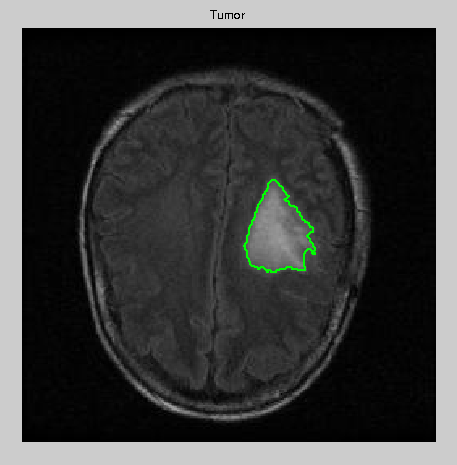
\includegraphics[width=0.5\textwidth]{images/2-tumeur-rand.png}
			\caption{Contours de la tumeur}
			\label{fig:fcm_tumeur_rand}
		\end{figure}
	% subsection avec_une_initialisation_al_atoire (end)


\section{Influence des paramètres} % (fold)
\label{sub:influence_des_param_tres}
	\subsection{Influence de l'indice de flou} % (fold)
	\label{ssub:influence_de_l_indice_de_flou}
		La figure \ref{fig:flou} représente la variation des ratios correspondant à l'augmentation de la surface de la tumeur pour différents indices de flous, en utilisant une initialisation aléatoire. On voit que ces résultats varient grandement. On sait cependant que la valeur 2 est celle conseillée, indépendamment de l'image, ces variations ne perturbent donc pas trop nos résultats puisque nous savons quelle valeur nous devons choisir.

		\begin{figure}[H]
			\centering
			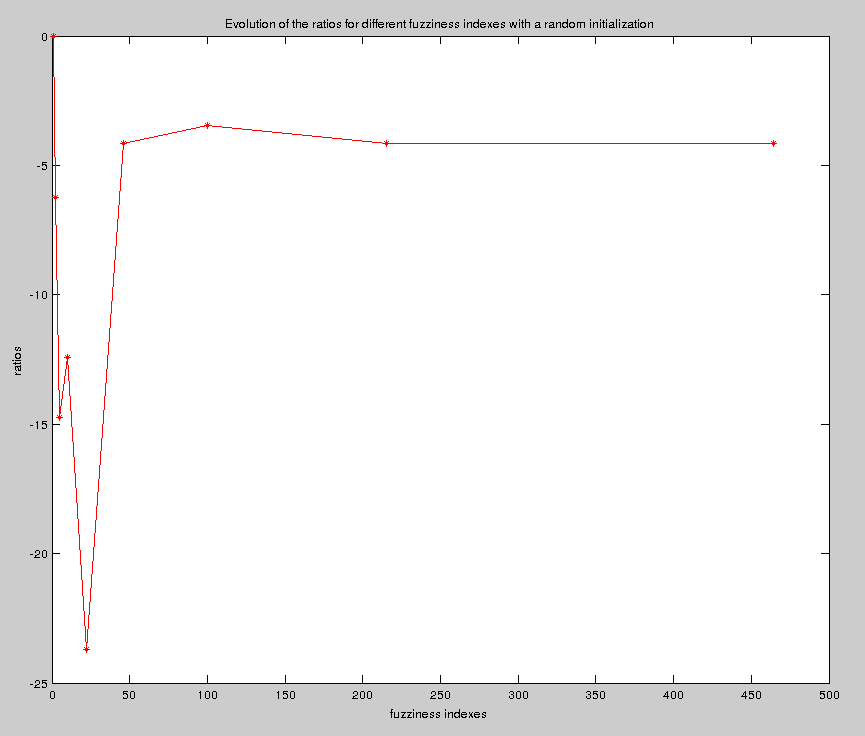
\includegraphics[width=0.7\textwidth]{images/2-flou.png}
			\caption{Influence de l'indice de flou sur le ratio d'augmentation de la surface de la tumeur}
			\label{fig:flou}
		\end{figure}
	% subsection influence_de_l_indice_de_flou (end)

	\subsection{Influence du epsilon} % (fold)
	\label{ssub:influence_du_epsilon}
		On appelle epsilon la variation maximum de la fonction de coût pour considérer que celle-ci est constante. Si la différence entre la fonction de coût à une itération avec celle de l'itération précédente est supérieure en valeur absolue à epsilon, on considère que l'algorithme n'a pas convergé et on continue, et dans le cas contraire on arrête. Plus epsilon est petit et plus on va effectuer d'itération, le résultat sera donc plus précis mais plus long à obtenir.\\

		Différente valeurs d'epsilon ont été testées. Les résultats sont présentés dans le tableau suivant :\\

		\begin{tabular}{|c|c|c|c|}
			\hline
			epsilon & temps d’exécution & nombre d'itérations & ratio d'augmentation \\ \hline
			$10^{-8}$ & 1.39 secondes & 45 & -6.23 \\
			$10^{-7}$ & 1.04 secondes & 43 & -6.23 \\
			$10^{-6}$ & 0.795 secondes & 40 & -6.23 \\
			$10^{-5}$ & 0.779 secondes & 38 & -6.23 \\
			$10^{-4}$ & 0.754 secondes & 35 & -6.23 \\
			$10^{-1}$ & 0.724 secondes & 31 & -6.23 \\
			\hline
		\end{tabular}
		\bigskip

		On remarque que le ratio ne change pas lorsqu'on change epsilon en restant dans des valeurs raisonnables. Cependant le temps d'exécution diminue. Une valeur d'epsilon d'environ $10^{-5}$ parait adaptée, puisque pour des valeurs plus grandes le temps de calcul diminue peu, et même si les ratios sont les mêmes pour ces images il parait plus prudent de rester précis.

	% subsection influence_du_epsilon (end)
% section influence_des_param_tres (end)
